\documentclass{article}
\usepackage[UTF8]{ctex}
% Replace `letterpaper' with`a4paper' for UK/EU standard size
\usepackage[a4paper,top=2cm,bottom=2cm,left=3cm,right=3cm,marginparwidth=1.75cm]{geometry}

% Useful packages
\usepackage{amsmath}
\usepackage{mathrsfs,amsmath}
\usepackage{graphicx}
\usepackage[colorlinks=true, allcolors=blue]{hyperref}
\usepackage{graphicx} %插入图片的宏包
\usepackage{float} %设置图片浮动位置的宏包
\usepackage{subfigure} %插入多图时用子图显示的宏包
\usepackage{parskip}
\usepackage{indentfirst} 
\setlength{\parindent}{2em}
\usepackage{hyperref}  
\usepackage{tikz}
\allowdisplaybreaks
\usepackage{multirow}
\usepackage{amsmath}
\usepackage{amsfonts,amssymb} 
\usepackage{xcolor} % 用于显示颜色
\usepackage{listings} % 用于插入代码
\lstset{
	basicstyle          =   \sffamily,          % 基本代码风格
	keywordstyle        =   \bfseries,          % 关键字风格
	commentstyle        =   \rmfamily\itshape,  % 注释的风格,斜体
	stringstyle         =   \ttfamily,  % 字符串风格
	flexiblecolumns,                % 别问为什么,加上这个
	numbers             =   left,   % 行号的位置在左边
	showspaces          =   false,  % 是否显示空格,显示了有点乱,所以不现实了
	numberstyle         =   \zihao{-5}\ttfamily,    % 行号的样式,小五号,tt等宽字体
	showstringspaces    =   false,
	captionpos          =   t,      % 这段代码的名字所呈现的位置,t指的是top上面
	frame               =   lrtb,   % 显示边框
}

\lstdefinestyle{Python}{
	language        =   Python, % 语言选Python
	basicstyle      =   \zihao{-5}\ttfamily,
	numberstyle     =   \zihao{-5}\ttfamily,
	keywordstyle    =   \color{blue},
	keywordstyle    =   [2] \color{teal},
	stringstyle     =   \color{magenta},
	commentstyle    =   \color{red}\ttfamily,
	breaklines      =   true,   % 自动换行,建议不要写太长的行
	columns         =   fixed,  % 如果不加这一句,字间距就不固定,很丑,必须加
	basewidth       =   0.5em,
}

\title{数据结构 lab-8 报告}
\author{林子开 21307110161}
\begin{document}
	\maketitle
	\tableofcontents
\section{算法思路说明}
首先,题目提供的是工序流程图,是有向无环图,各个节点的最长或最短距离的更新关系是确定的。
因此,可以先对图进行\textbf{拓扑排序},然后基于拓扑序进行距离计算。其中,拓扑排序基于深度优先搜素完成。
该部分的算法复杂度为$\mathcal{O}(V+E)$

其次,虽然题目要求找的是最长带权距离,但如果将所有的边的权重都取成相反数,也即$(u,v,w)\rightarrow(u,v,-w)$,
那么,\textbf{问题等价于求权重取相反数后的图的最短路径}。因此,仍然可以使用基于拓扑序求有向无环图最短路径的算法,
找到权重取反后的图的“最短的”路径。最后计算距离时,再将该路径长度取相反数,即可得到最长路径距离。
该部分的复杂度为$\mathcal{O}(V+E)$。

总的算法复杂度为$\mathcal{O}(V+E)$。

\section{Python代码主要功能介绍}
在文件\texttt{find-longest-path.py}文件中,我定义了两个类,分别是表示图节点的\texttt{vertex}类,
和表示有向图的\texttt{Graph}类。

在\texttt{Graph}中,基于深度优先搜索(\texttt{DFS}方法)实现了
拓扑排序(\texttt{topologicalSort}方法)。基于拓扑排序的结果,实现了\texttt{findShortestPath}方法,
该方法能够找到图中从起点开始到达所有其他点的最短路径。

最后,实现了\texttt{findLongestPath}方法,该方法先将图中所有边的\textbf{权重取相反数},然后调用\texttt{findShortestPath}
找到权重取反后的图的“最短”路径(也即原图的最长路径),并将该路径,以及路径对应的长度返回。

\texttt{criticalPath}是辅助性的函数,用于格式化地建立\texttt{Graph}实例,并打印路径和路径长度。

\section{测试用例实验结果}
说明:由于题目只要求\textbf{找出一条}最长的带权路径,因此以下给出的答案可能不唯一。
\subsection{测试用例1}
% 测试用例1如下如下:
\begin{figure}[H]
	\centering
	{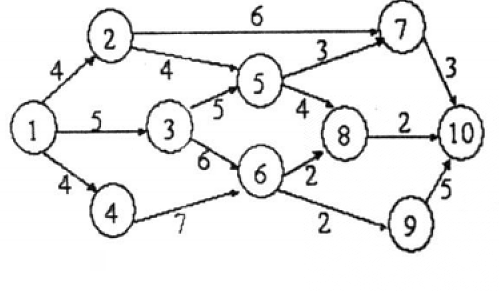
\includegraphics[width=0.5\textwidth]{example1.png}} 
	\caption{测试用例1的示意图} 
\end{figure}
最长路径:1$\;\longrightarrow \; $ 4$\;\longrightarrow \; $ 6$\;\longrightarrow \; $ 9$\;\longrightarrow \; $ 10。路径长度为:18。

\subsection{测试用例2}
% 测试用例2如下如下:
\begin{figure}[H]
	\centering
	{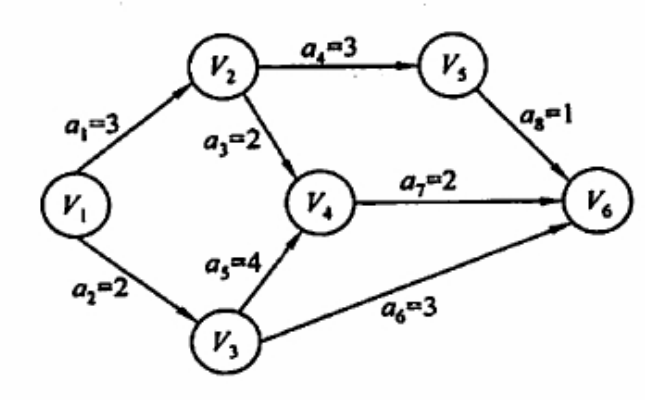
\includegraphics[width=0.5\textwidth]{example2.png}} 
	\caption{测试用例2的示意图} 
\end{figure}
最长路径:V1$\;\longrightarrow \; $ V3$\;\longrightarrow \; $ V4$\;\longrightarrow \; $ V6。路径长度为:8。

\subsection{测试用例3}
% 测试用例3如下如下:
\begin{figure}[H]
	\centering
	{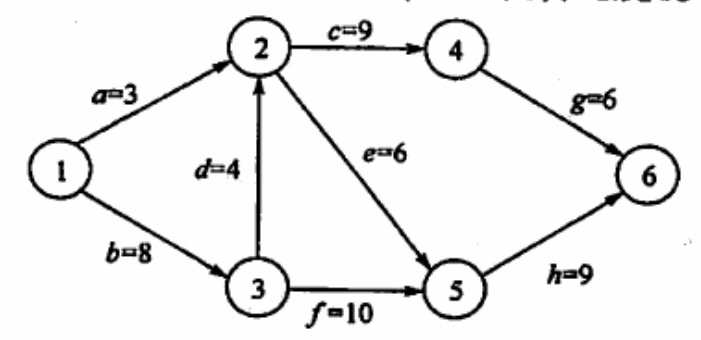
\includegraphics[width=0.5\textwidth]{example3.png}} 
	\caption{测试用例3的示意图} 
\end{figure}
最长路径:1$\;\longrightarrow \; $ 3$\;\longrightarrow \; $ 5$\;\longrightarrow \; $ 6。路径长度为:27。

\subsection{测试用例4}
% 测试用例4如下如下:
\begin{figure}[H]
	\centering
	{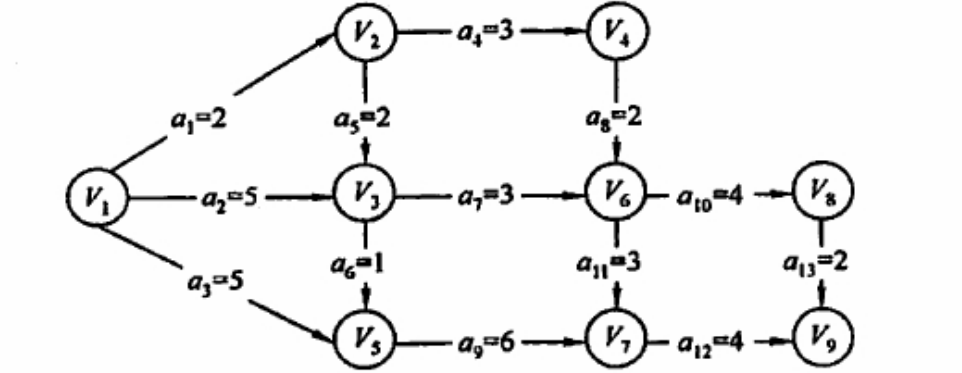
\includegraphics[width=0.5\textwidth]{example4.png}} 
	\caption{测试用例4的示意图} 
\end{figure}
最长路径:V1$\;\longrightarrow \; $ V3$\;\longrightarrow \; $ V5$\;\longrightarrow \; $ V7$\;\longrightarrow \; $ V9。路径长度为:16。



\end{document}

% \begin{figure}[H]
% 	\centering
% 	{\includegraphics[width=0.35\textwidth]{image//ignorance.png}} 
% 	\caption{} \label{} 
% \end{figure}


% \lstinputlisting[style = Python,
% caption={Python codes},
% label = {efficient},
% linerange={110-125}]{exercise3.py} 


% \begin{figure}[H]
%     \centering
%     \subfigure[patch size = 11]
%     {\label{} \includegraphics[width=0.49\textwidth]{image//local equalization with patch size = 11.jpg}}
%     \,    
%     \subfigure[patch size = 51]
%     {\label{} \includegraphics[width=0.49\textwidth]{image//local equalization with patch size = 51.jpg}}
%     \,
%     \subfigure[patch size = 151]
%     {\label{} \includegraphics[width=0.49\textwidth]{image//local equalization with patch size = 151.jpg}}
%     \,    
%     \subfigure[patch size = 201]
%     {\label{} \includegraphics[width=0.49\textwidth]{image//local equalization with patch size = 201.jpg}}
%     \caption{local equalization with different patch sizes}\label{} 
% \end{figure}
